\scanpage{8}
\diagram{\begin{tikzcd}
M\arrow[r,"V"]\arrow[d,"V"]&M^{(p)}\arrow[d,"V^{(p)}"]\\
M^{(p)}\arrow[r,"V^{(p)}"]\arrow[u,bend left=45,"F"]&M^{(p^2)}\arrow[u,bend left=35,"F^{(p)}"]
\end{tikzcd}}
\[
\unsure{V^\vee}\quad F
\]
\[
M
\]
$(\mathrm I)$
\diagram{\begin{tikzcd}&B\arrow[dl,"\partial_{\mathrm I}"']&\\A\arrow[rr,"i_{\mathrm I}"]&&\unsure{\mathfrak X|\mathcal X}^{p}\arrow[ul,"\pi_{\mathrm I}"']\end{tikzcd}}
$(\mathrm {II})$
\diagram{\begin{tikzcd}&A\arrow[dl,"\partial_{\mathrm {II}}"']&\\B\arrow[rr,dash,"i_{\mathrm {II}}"]&&\mathfrak X\arrow[ul,"\pi_{\mathrm {II}}"']\end{tikzcd}}
$(\mathrm {II}^{(p)})$
\diagram{\begin{tikzcd}&A^p\arrow[dl,"\partial_{\mathrm {II}}^{(p)}"']&\\B^p\arrow[rr,"i_{\mathrm {II}}^{(p)}"']&&\mathfrak X^p\arrow[ul,"\pi_{\mathrm {II}}^{(p)}"']\end{tikzcd}}
\[
\boxed{\begin{array}{ll}
\unsure{i_{\mathrm {II}}}\pi_{\mathrm I}:&\mathfrak X^p\overset{F_{\mathfrak X}}{\mathbin{-}}\mathfrak X\\
i_{\mathrm I}\pi_{\mathrm {II}}:&\mathfrak X\xrightarrow{V_{\mathfrak X}}\mathfrak X^p
\end{array}}
\]
\[
\boxed{\left\{\begin{array}{ll}
\partial_{\mathrm I}\partial_{\mathrm {II}}:&A^{\deleted{\unsure{a}}}\xrightarrow{2}A\quad\text{nul?}\\
\partial_{\mathrm {II}}\partial_{\mathrm I}:&B^{\deleted{\unsure{a}}}\xrightarrow{2}B\quad\text{nul?}\\
\pi_{\mathrm {II}}^{(p)}i_{\mathrm I}:&A\xrightarrow{V_A}A^{(p)}\\
\pi_{\mathrm I}\deleted{\unsure{\mu}}\,i_{\mathrm {II}}^{(p)}:&B^{(p)}\overset{F_B}{\mathbin{-}}B^{\deleted{\unsure{(p)}}}
\end{array}\right.}
\]
\figure{\begin{tikzpicture}[x=1cm,y=1cm]
\draw (0,3) ellipse (.65 and .27);\node at (0,3){nul?};
\draw (0,2.3) ellipse (.65 and .27);\node at (0,2.3){nul?};
\draw[->] (-1.8,3.7)--(-3.9,3.6);
\draw[->] (-3.5,1)--(-3.7,3.5);
\draw[->] (-3.4,.8)--(-1.9,.9);
\draw[->] (-3.8,-2.3) to[bend left=30] (-3.6,.9);
\draw[->] (-3.95,-2.2) to[bend left=30] (-3.65,1.15);
\draw (-3.85,.9)--(-3.6,1.2)--(-2.9,.9);
\node at (-3.8,.35){$\unsure{\mu}$};
\end{tikzpicture}}

$\varphi^*(\mathrm {III})\simeq(\mathrm I^{\unsure{?}})$
\diagram{\begin{tikzcd}
&\varphi^*(\unsure{b})\arrow[dl,"(\partial_{\mathrm I}\simeq\varphi^*(\partial_0))"']&\\
\varphi^*(a)\unsure{A}\arrow[rr,"(i_{\mathrm I}=\varphi^*(i_0))"]&&\mathfrak X^p\arrow[ul,"(\pi_{\mathrm I}\simeq\varphi^*(\pi_0))"']
\end{tikzcd}}
$\mathrm {III}$
\diagram{\begin{tikzcd}&b\arrow[dl,"\partial_0"']&\\a\arrow[rr,dash,"i_0"]&&\mathfrak X\arrow[ul,"\pi_0"']\end{tikzcd}}
\figure{\begin{tikzpicture}\draw (0,1.5)--(7,1.8);\draw(0,0)--(5.4,.2);\draw(4.8,0)--(4.8,1.7);\end{tikzpicture}}

\diagram{\begin{tikzcd}[column sep=small,row sep=small]
&0\arrow[r,dash]\arrow[d,dash]&M\arrow[r]\arrow[d]&M^p\arrow[r,dash]\arrow[d]&\unsure{\cdot}\\
&M^p\arrow[r,dash]\arrow[d]&M\arrow[r,dash]\arrow[d,dash]&0\arrow[r,dash]\arrow[d,dash]&{}\\
M\arrow[r,dash]&M^p\arrow[r,dash]&\unsure{0}\arrow[r,dash]&\unsure{\cdot}&
\end{tikzcd}}
$\varepsilon^*(\mathrm I)\simeq\mathrm {III}^{(p)}$
\diagram{\begin{tikzcd}&b^p\arrow[dl,"\partial_0^{(p)}"']&\\a^p\arrow[rr,dash,"i_0^{(p)}"]&&X^p\arrow[ul,"\pi_0^{(p)}"']\end{tikzcd}}
$\varepsilon^*(\mathrm {II}):$
\diagram{\begin{tikzcd}&a^p\arrow[dl,"\varepsilon^*(\partial_{\mathrm {II}})"']&\\b^p\arrow[rr,"\varepsilon^*(i_{\mathrm {II}})"']&&X\arrow[ul,"\varepsilon^*(\pi_{\mathrm {II}})"']\end{tikzcd}}
\margin{$\left.\begin{array}{c}\phantom{a}\\\phantom{a}\\\phantom{a}\end{array}\right\}$ triangles compatibles avec $F-V$ structures}

\deleted{$\unsure{\partial_0\varepsilon^*}$}
\[
\boxed{\left\{\begin{array}{ll}
\pi_0\varepsilon^*(i_{\mathrm {II}}):&b^{(p)}\xrightarrow{F_b}b\\\hline
\deleted{\unsure{\partial}}\varepsilon^*(\pi_{\mathrm {II}})i_0:&a\xrightarrow{V_a}a^{(p)}
\end{array}\right.}
\]
\figure{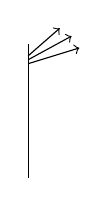
\begin{tikzpicture}\draw (0,0)--(0,1.7);\draw[->](0,1.55)--(.4,1.9);\draw[->](0,1.5)--(.55,1.8);\draw[->](0,1.45)--(.65,1.65);\end{tikzpicture}}
\diagram{\begin{tikzcd}\mathfrak X^p\arrow[r,dash]&B\arrow[r,dash]&\mathfrak X\end{tikzcd}}
\diagram{\begin{tikzcd}\mathfrak X\arrow[r,dash]&A\arrow[r,dash]&\mathfrak X^{(p)}\end{tikzcd}}
\diagram{\begin{tikzcd}X^{(p)}\arrow[r]&b^{(p)}\arrow[r,dash]&X\end{tikzcd}}
\diagram{\begin{tikzcd}X\arrow[r,dash]&a^{(p)}\arrow[r,dash]&X^{(p)}\end{tikzcd}}
\mspage{7}
